\documentclass[12pt]{article}
\usepackage[french]{babel}
\usepackage[T1]{fontenc}
\usepackage{listings}
\usepackage{amsmath,amsthm,amssymb,amsfonts}
\usepackage[dvipsnames]{xcolor}
\usepackage{pgfpages}
\usepackage{fullpage}
\usepackage[unicode,psdextra]{hyperref}
\usepackage{graphics}
\usepackage{float}
\usepackage{fancyvrb}

%---------------------------------------%
%             Paramétrage               %
%---------------------------------------%

\lstdefinestyle{codeblock}{
	keywordstyle=\color{magenta},
	basicstyle=\ttfamily\footnotesize,
	identifierstyle=\color{blue},
	numbersep=5pt,
	tabsize=2,
	breaklines=true,
	numbers=left,
	captionpos=b,
	frame=single
}
\lstset{style=codeblock}

\hypersetup{
	colorlinks,
	citecolor=black,
	filecolor=black,
	linkcolor=black,
	urlcolor=black
}

%---------------------------------------%
%         Information  Générale         %
%---------------------------------------%

\title{Rapport de projet\\ Platformer}
\author{\small FARGEAT Alexis, MAGNIN Mathis, VERDIER Vincent}

%---------------------------------------%
%                Document               %
%---------------------------------------%

\begin{document}

	\maketitle

	\begin{figure}[H]
		\centering
		\begin{BVerbatim}
 _____  ______                               
|  __ \|  ____|                             
| |__) | |__ ___  _ __ _ __ ___   ___ _ __   
|  ___/|  __/ _ \| '__| '_ ` _ \ / _ | '__|
| |    | | | (_) | |  | | | | | |  __| |     
|_|    |_|  \___/|_|  |_| |_| |_|\___|_|   


		\end{BVerbatim}
	\end{figure}

	\tableofcontents
	\newpage

	\section{Introduction}
	
		\begin{center}
			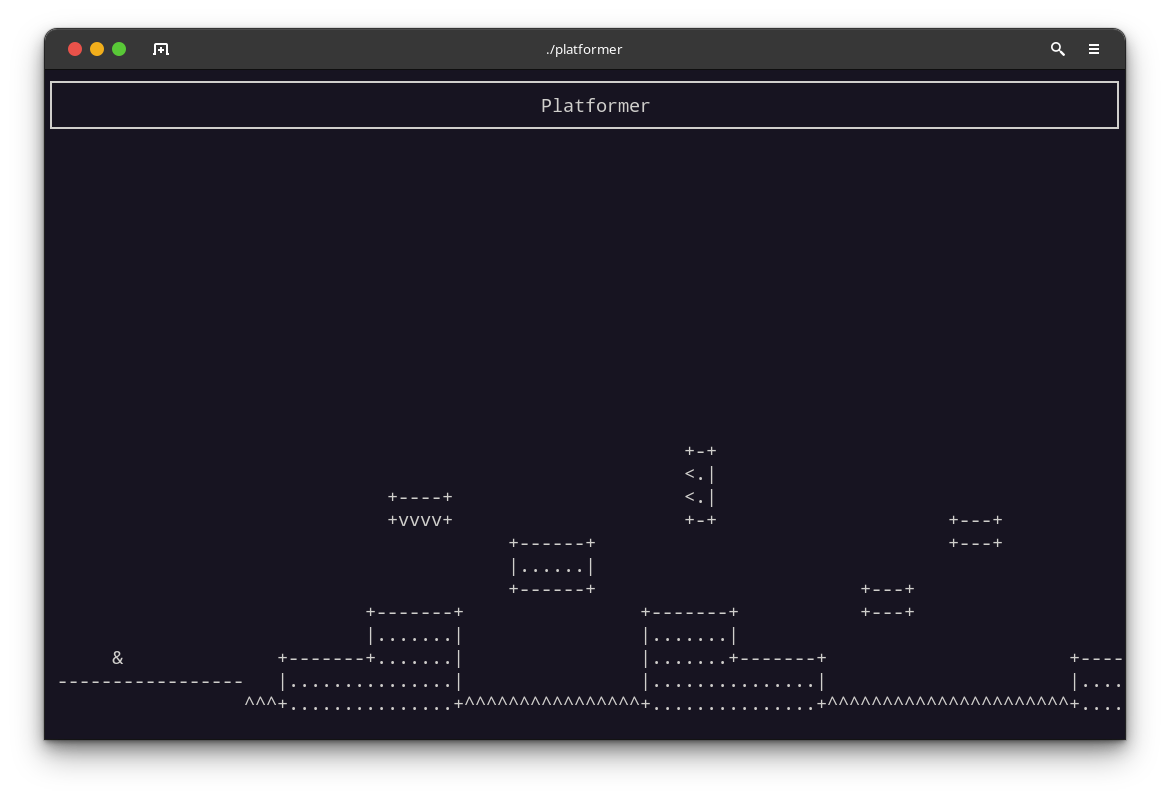
\includegraphics[width=0.90\textwidth]{content/image.png}
		\end{center}
	
		Platformer est un jeu de plateforme, où le but est d'arriver au bout d'une carte après de multiple obstacles.
		Ce jeu se rapproche de Mario Bros.
	
		Le jeu est programmé en \textbf{C} et s'utilise dans une console (similaire a MS-DOS).
	

	\section{Problèmes recontrés}

		\subsection{Chargement de la carte}
		
			Au cours de la création du jeu, il a fallu choisir une manière de stocker les données de la carte du jeu.\\


			Nous cherchions une solution permettant un accès simple par les autres parties du programme comme l’affichage.
		
			Nous voulions également avoir la possibilité de modifier la carte du jeu de manière visuelle et sans recompiler le jeu.\\


			Cela nous a amené à choisir de stocker la carte dans un fichier texte qui sera chargé dans le jeu sous forme 
			d’un tableau à deux dimensions de taille dynamique.\\
		
			Au lancement du jeu, les données du fichier texte sont lues et la taille du tableau à allouer est calculée en 
			comptant le nombre de caractères de la ligne du haut de la carte.\\
		
			On stocke alors dans une structure  :
			\begin{itemize}
				\item Les dimensions (x, y) de la carte
				\item Un tableau contenant les données du fichier texte
				\item Un autre tableau utile pour les collisions dont le fonctionnement est détaillé dans la partie Collisions.
				\item \dots\\
			\end{itemize}
		
			Un tableau en 2D de taille dynamique nécessite de libérer la mémoire occupée celui-ci l’arrêt du programme.
		
			Un tableau en 2D peut être vu comme un tableau en 1D stockant des pointeurs qui pointent le premier élément 
			de chaque colonne. Ce tableau en 1D correspond à la première ligne du tableau en 2D.
		
			Pour libérer la mémoire occupée par le tableau on libère d’abord la mémoire occupée par chaque colonne puis 
			on libère la mémoire occupée par la première ligne.
		
	
		\subsection{Physique et mouvement}
		
		\subsection{Affichage}
		
		\subsection{Collisions}
		
		
		\begin{lstlisting}[language=C, title={Programme en C}]
			int test;
		\end{lstlisting}

	\section{Conclusion}

	Parmi les idées qui auraient pû améliorer le jeu, nous avons retenu :
	\begin{itemize}
		\item Un menu pour choisir la carte
		\item Des adversaires automatiques
		\item Des couleurs
		\item Éventuellement, un outil pour créer d'autres cartes (ou un guide)
		\item \dots
	\end{itemize}
		
\end{document}